%!TEX root = ../dissertation.tex
\chapter{Introduzione}
\label{introduction}
Il seguente capitolo si pone l'obiettivo di presentare il contesto in cui si è svolto lo stage. \\
Viene fornita una descrizione dell’azienda, della sua struttura e dei clienti a cui si rivolge. \\
Inoltre vengono illustrate le tecnologie che vengono utilizzate dall'azienda e che sono state impiegate nel corso dello stage.

\section{L'azienda}
NETCOM nasce nel 1999 con l’obiettivo di proporre al mercato soluzioni e servizi di eccellenza per l’\gl{IT Life Cycle Management} e l’\gl{IT Governance}. Quest’ultimo, viene inteso dall’azienda come l’insieme dei processi, procedure, competenze e strumenti utili alla gestione degli item che compongono il sistema informativo, in tutte le fasi del loro ciclo di vita, per gli aspetti di:
\begin{itemize}
    \item Gestione tecnica: per la soluzione di problemi di qualsiasi natura che il cliente può riscontrare nell’utilizzo del sistema;
    \item \emph{Governance}: per la gestione di tutte le operazioni IT di livello manageriale ed allinearle alle richieste del business.
\end{itemize}

L'\emph{IT Life Cycle Management} è un \gl{framework} che si occupa di gestire e ottimizzare il sistema informativo di un'organizzazione, riducendo costi e rischi e aumentando complessivamente la qualità. Per questo motivo, il personale NETCOM del settore tecnico, vanta certificazioni di \gl{best practices}( \gl{ITIL} Foundation e ITIL Intermediate) e standard (ISO 9001 e ISO 20000) per la gestione del sistema informativo.  Essendo partner \emph{Ivanti, SNOW} ed \emph{EasyVista}, il personale NETCOM presenta certificazioni che attestano la competenza operativa nei rispettivi \emph{software}. \cite{itil-pro} \\


\begin{figure}[H]
    \centering
    \captionsetup{justification=centering,margin=2cm}
        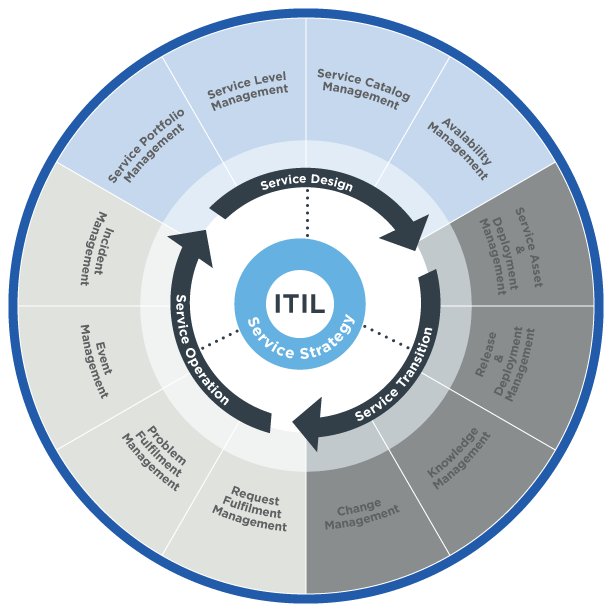
\includegraphics[width=0.5\textwidth ]{figures/itil.png}
        \caption [ITIL framework]{ ITIL framework \label{fig:myInlineFigure}}
\end{figure}

La tipologia dei principali servizi offerti da NETCOM colloca l’azienda nel mercato delle soluzioni di \emph{System Management}, settore dedicato alla gestione di tutti gli elaboratori presenti all’interno di un’organizzazione.\\
Gli aspetti a cui l'azienda pone maggior attenzione riguardano attività come la distribuzione dello strato \emph{software} destinato all’utilizzo di un dato \emph{host}, l’installazione distribuita di applicazioni, la gestione remota di aggiornamenti e vulnerabilità, l’inventario dello stato e della configurazione delle macchine all’interno dell’organizzazione e il controllo remoto degli \emph{host}.
L'azienda offre una vasta gamma di servizi che ne determinano la competitività:
\begin{itemize}
\item \emph{Software Asset Management}: servizio di consulenza che consente di comprendere quante e quali delle licenze \emph{software} acquistate sono effettivamente necessarie in funzione dell'utilizzo del cliente e delle relative strategie di business. Il \gl{SAM} è un approccio strutturato che si basa su una serie di processi, \textit{best practices} e competenze specifiche, il cui obiettivo è di ridurre le complessità di gestione, i rischi ed i costi effettivi del \emph{software}.\\
NETCOM offre servizi multilivello volti a proteggere e valorizzare il patrimonio \emph{software} delle organizzazioni, affiancandole nelle verifiche di conformità e nell’ ottimizzazione relativamente al contesto operativo;
\item  \emph{IT Service Management}: servizio che si occupa della modellazione dei servizi IT tracciando le linee guida per la progettazione e la realizzazione dei sistemi per l’automazione dei processi relativi ai servizi aziendali. Attraverso un ciclo costante di monitoraggio, \emph{reporting} e revisione dei risultati dei servizi IT, il personale NETCOM è in grado di indicare al management i provvedimenti da attuare per eliminare i livelli di servizio inefficienti;
\item \emph{IT Asset Management}: servizio costituito da un insieme di \textit{best practices}, processi e strumenti che permettono alle funzioni amministrative, contrattuali e di inventario di supportare la corretta gestione del ciclo di vita degli \gl{asset}. \\ 
NETCOM collabora con i clienti analizzando le richieste dei singoli dipartimenti e, coerentemente con strategie di business, progetta ed implementa la gestione dei processi di \emph{Asset Management};
\item Assistenza tecnica: servizio che garantisce la continuità nel funzionamento del sistema di management e coadiuva il personale del cliente nel caso in cui si presentino problematiche durante l’utilizzo quotidiano della soluzione. NETCOM offre la possibilità di stipulare contratti annuali di assistenza tecnica che prevedono l'utilizzo di strumenti evoluti, i quali ne garantiscono l'efficacia. Tutti i problemi \emph{software} sono poi risolti da remoto nel pieno rispetto della sicurezza aziendale. \cite{netcom-info}
\end{itemize}
\section{Organizzazione aziendale}
NETCOM conta circa 30 dipendenti con sede principale a Padova, in via Fusinato 42. 
Lo stage è stato svolto all’interno del dipartimento di \emph{Development}, che si occupa dello sviluppo di soluzioni proprie interne all’azienda. \\ L'organizzazione aziendale interna può essere schematizzata dal seguente organigramma: 
\begin{figure}[H]
    \centering
    \captionsetup{justification=centering,margin=2cm}
        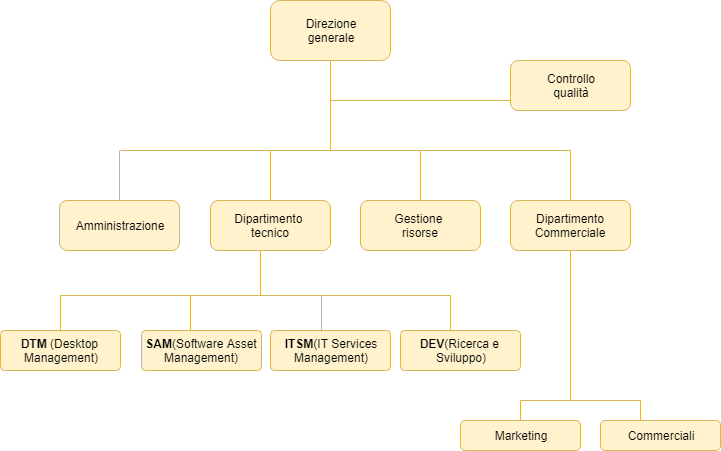
\includegraphics[width=0.8\textwidth ]{figures/schemaaziendale}
        \caption [Organizzazione aziendale NETCOM]{ Organizzazione aziendale NETCOM \label{fig:organigramma}}
\end{figure}
\begin{itemize}
    \item Direzione Generale: si occupa della pianificazione e organizzazione di tutte le attività dell’azienda;
    \item Controllo Qualità: definisce il sistema di qualità aziendale aderendo agli standard ISO e a \textit{best practices} seguiti dall'azienda;
    \item Amministrazione: gestisce l’infrastruttura e la contabilità dell’azienda;
    \item Gestione Risorse: gestisce le risorse umane;
    \item Dipartimento Tecnico: composto da quattro sotto dipartimenti, è la parte dell’azienda che eroga concretamente i servizi.
\end{itemize}

\section{Target}
NETCOM lavora con più di 150 clienti distribuiti su tutto il territorio nazionale, di diverse tipologie e dimensioni, attive sia nel settore privato che nel settore pubblico. 
Per le caratteristiche dei servizi offerti, NETCOM si rivolge alla medio-grande impresa italiana che possiede tra i 250 e i 10000 dispositivi. Considerando l'ampia gamma di servizi che NETCOM offre attualmente , essa è adeguata per diverse tipologie di clientela come ad esempio le aziende che ricercano una garanzia di funzionamento o le aziende che desiderano investire in soluzioni di \emph{System Management} e di sicurezza. 
Analizzando i principali servizi proposti da NETCOM, è possibile individuare il tipo di clientela a cui si rivolgono:
\begin{itemize}
    \item Assistenza Tecnica : è un servizio di base che viene erogato al momento del bisogno, ovvero quando, durante l'utilizzo di un sistema informativo, si presentano alcune problematiche che vanno al di là della competenza del reparto IT dell’azienda del cliente. 
    Per evitare i rischi derivanti dalla loro scarsa competenza tecnica, il personale esperto e certificato garantisce la risoluzione del problema, facendo in modo che il cliente possa concentrarsi sul \emph{business}.
    Questo servizio, non richiedendo onerosi investimenti iniziali, è adatto alle aziende che hanno un budget limitato per il reparto informatico;
    \item \emph{Desktop Management}: è un servizio che si occupa di permettere a un’impresa il controllo gestionale del proprio sistema informativo tramite l’installazione dei prodotti che essa offre e tramite corsi di formazione per il personale del cliente. Questo tipo di servizio costituisce una spesa più onerosa rispetto alla semplice assistenza su richiesta e può essere visto come una scelta lungimirante. 
    Le aziende a cui può interessare questo servizio, sono quelle che desiderano provare qualcosa di innovativo accettando il rischio dell’investimento iniziale e il compromesso di gestire autonomamente il loro \emph{asset} tramite gli strumenti e la formazione offerta da NETCOM;
    \item \emph{Asset Management} Automatizzato: è il servizio più completo, poiché sono gli operatori di NETCOM a svolgere tutte le attività riguardanti la gestione del sistema informativo di un’organizzazione.
    Questo servizio si rivolge a entrambe e tipologie di aziende sopra individuate: le imprese che vogliono innovarsi e che approvano la spesa iniziale puntando ad avere un ritorno economico futuro; le imprese che vogliono mantenere la loro attuale situazione ma hanno l’esigenza di delegare a qualcuno la gestione del loro sistema informativo;
    \item \emph{Self Service Password Management}: la gestione automatizzata del cambio e del \emph{reset} della password può risultare di utilità fondamentale alle aziende che intendono garantire maggiore sicurezza alla propria organizzazione, grazie all’individuazione precisa dell’identità dell’utente che richiede il ripristino della password. Inoltre si presenta adatta alle aziende con \gl{help desk} che desiderano affidare ad un \emph{software} la gestione delle password, ma allo stesso tempo necessitano del rispetto totale dei requisiti di sicurezza richiesti dalle aziende di medio-grandi dimensioni;
    \item \emph{Software Asset Management}: questo servizio si occupa della gestione dell’intero ciclo di vita del \emph{software}, dall’implementazione fino alla sua ritiro.
    NETCOM si occupa di verificare la conformità del \emph{software} installato rispetto alle licenze acquistate e permette l’elaborazione di una strategia di normalizzazione, che prevede l’acquisizione, rimozione o sostituzione di alcuni applicativi, al fine di garantire.
    Questo servizio essere considerato utile ad un’azienda che è stata sottoposta ad una verifica formale del proprio \emph{asset software}, ma anche di un’azienda che vuole ridurre gli sprechi, assicurandosi la propria compliance rispetto alle licenze acquistate e mantenendo la garanzia di funzionamento del sistema informativo.
\end{itemize}
NETCOM offre un’ampia gamma di soluzioni per le aziende che necessitano sia di garanzie di funzionamento sia di proposte innovative, offrendo un servizio completo alla propria clientela.
Inoltre la conformità del proprio \emph{asset} \emph{software} alle licenze acquistate, si rivela un servizio necessario sia in caso di \gl{audit}, sia in caso di bisogno da parte del cliente di focalizzarsi sul proprio business lasciando a NETCOM la gestione dei degli applicativi da acquisire e installare. \cite{netcom-info}

\section{Tecnologie} 
Dal momento che NETCOM è una società che offre principalmente servizi di consulenza, è necessario distinguere le tecnologie utilizzate dall'azienda e quelle a supporto dello stage.
Alla studentessa è stato richiesto di utilizzare le tecnologie usualmente impiegate dal reparto Ricerca e Sviluppo dell'azienda, che differiscono da quelle quotidianamente adoperate dall’azienda per erogare i propri servizi di \emph{Desktop Management, Asset Managemen}t e \emph{Software Asset Management}.
\subsection{Utilizzate dall'azienda}
Nell'ambito della consulenza, NETCOM fa uso principalmente delle seguenti tecnologie:
\begin{itemize}
    \item \emph{Ivanti Endpoint Management}: soluzione, illustrata in Figura 1.3, di gestione dei dispositivi fissi e mobili degli utenti, che attraverso un’unica console centralizzata, consente di monitorare lo stato dei device, distribuire \emph{software/patch} di sicurezza ed automatizzare azioni correttive per garantirne la sicurezza e l'affidabilità;
        \begin{figure}[!ht]
        \centering
        \captionsetup{justification=centering,margin=2cm}
            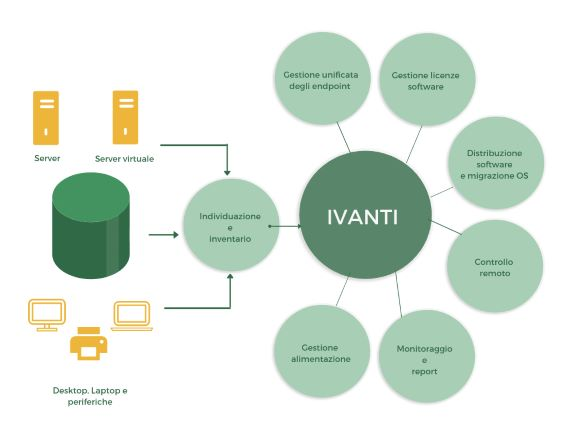
\includegraphics[width=0.6\textwidth ]{figures/Ivanti.png}
            \caption [Ivanti]{Ivanti \label{fig:Ivanti}}
    \end{figure}
    \item \emph{EasyVista}: soluzione \emph{software} di \gl{ITSM} altamente personalizzabile, pensata per realtà aziendali altamente strutturate e che necessitano di un alto grado di allineamento con il \emph{framework ITIL}. Essendo un \emph{software} integrato e modulare, è in grado di ottimizzare la gestione IT migliorando la qualità dei servizi e mantenendo sotto controllo i costi.
    Tra le funzionalità principali di \emph{EasyVista} figurano:
    \begin{itemize}
        \item Apertura di \gl{ticket} riguardanti incidenti e richieste di servizio;
        \item Gestione da parte del reparto tecnico di tutti i \emph{ticket} e assegnazione alle persone competenti per una risoluzione rapida e definitiva di essi;
        \item Amministrazione degli \emph{asset} aziendali.
    \end{itemize}
    \begin{figure}[t]
        \centering
        \captionsetup{justification=centering,margin=2cm}
            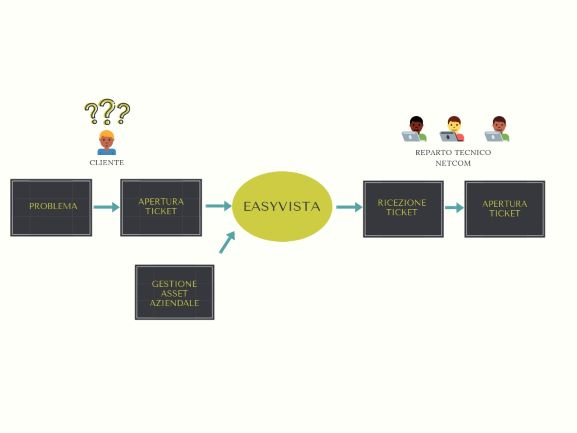
\includegraphics[width=0.6\textwidth ]{figures/easyvista.jpg}
            \caption [EasyVista]{Visione ad alto livello del funzionamento di EasyVista \label{fig:EasyVista}}
    \end{figure}
    \item \emph{Snow License Manager}: piattaforma di \emph{Software Asset Management}, in grado di raccogliere i dati sulle applicazioni installate di computer e dispositivi mobili, determinare automaticamente lo stato di conformità delle licenze ed ottimizzarne l'assegnazione in base alla raccolta dei dati di effettivo utilizzo degli applicativi. La soluzione è progettata per ridurre i rischi, i costi e la complessità associati alla gestione del \emph{software}, evitando gli sprechi per l’acquisto di licenze effettivamente inutilizzate e garantendo allo stesso tempo la piena conformità ai contratti d’uso.
    \emph{SNOW} permette la suddivisione del progetto di \emph{Software Asset Management} in tre attività principali:
    \begin{itemize}
        \item \emph{Assessment}: come prima attività, è indispensabile formalizzare i requisiti del cliente ed analizzare lo stato degli \gl{asset} da molteplici punti di vista (installazioni, utilizzo, licenze), per poter delineare la situazione attuale e le possibili strategie di normalizzazione;
        \item Normalizzazione: sulla base della strategia scelta, alcuni applicativi dovranno essere acquistati, rimossi, installati o sostituiti. L’attività di normalizzazione supporta il cliente nell’applicazione delle modifiche;
        \item Mantenimento: questa fase prevede una serie di attività di controllo ricorrenti al fine di garantire nel tempo gli obiettivi raggiunti.
    \end{itemize}
     \begin{figure}[h]
        \centering
        \captionsetup{justification=centering,margin=2cm}
            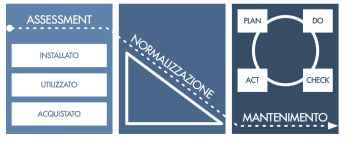
\includegraphics[width=0.6\textwidth ]{figures/snow.png}
            \caption [Snow License Manager]{Fasi del progetto di SAM gestite tramite SNOW \label{fig:snow}}
    \end{figure}   
    
    \item \emph{Hydrogen}: applicazione per permettere il \emph{self-reset} delle password dimenticate o scadute da parte degli utenti, incrementando la sicurezza e riducendo i costi per il servizio di \emph{help desk}. Tale servizio si integra completamente con l’interfaccia di accesso Windows (fase di richiesta login e password) aggiungendovi la funzionalità di \emph{reset} password. Hydrogen si propone come soluzione per aziende medio-grandi, in sostituzione all’identificazione dell’utente tramite il riconoscimento vocale da parte dell’operatore del servizio di \emph{help desk}, poiché è plausibile pensare che l’operatore non sia in grado di riconoscere chiunque unicamente dalla voce tramite una telefonata;
    
    \item \emph{Beryllium SPLA Manager}: soluzione che serve ad automatizzare la generazione di report, solitamente prodotti manualmente da personale tecnico specializzato, che individuano l'effettivo utilizzo del \emph{software}. Questo progetto si pone l'obiettivo di offrire ai \gl{service provider} uno strumento completo che consente di monitorare e gestire i contratti \gl{SPLA} stipulati.
\end{itemize}

\subsection{A supporto dello stage}
\subsubsection{\underline{Linguaggi}}
\begin{itemize}
    \item C \#: è un linguaggio di programmazione semplice, elegante e \emph{type-safe} sviluppato da Microsoft, che consente agli sviluppatori di creare una vasta gamma di applicazioni protette e affidabili per \emph{.NET Framework}. Essendo un linguaggio orientato a oggetti, C \# supporta i concetti di incapsulamento, ereditarietà e polimorfismo;\cite{microsoft-csharp}
    \item SQL: è un linguaggio standardizzato per \emph{database} relazionali progettato per creare e modificare schemi di \emph{database}; inserire, modificare e gestire dati memorizzati; interrogare i dati memorizzati; creare e gestire strumenti di controllo e accesso ai dati;\cite{db-sql}
    \item PowerShell: è una \emph{shell} caratterizzata dall'interfaccia a riga di comando e da un linguaggio di \emph{scripting}, sviluppata da Microsoft. È basato sulla programmazione a oggetti e sul \emph{framework} Microsoft .NET. PowerShell è la combinazione di compiti complessi e di una serie di componenti, le \emph{cmdlets}  (\emph{command lets}, serie di comandi), che sono classi .NET progettate per sfruttare le caratteristiche dell'ambiente. \cite{microsoft-ps}
\end{itemize}
\subsubsection{\underline{Framework}}
\begin{itemize}
    \item .NET Framework: è un ambiente di esecuzione gestita per Windows che fornisce un'ampia gamma di servizi alle \emph{app} in esecuzione. È costituito da due componenti principali: \emph{Common Language Runtime (CLR)}, vale a dire il motore di esecuzione mediante il quale vengono gestite le \emph{app} in esecuzione, e la libreria di classi .NET Framework, che fornisce una raccolta di codice testato e riutilizzabile che gli sviluppatori possono chiamare dalle rispettive \emph{app}.\cite{microsoft-net}
\end{itemize}
\subsubsection{\underline{Software di sviluppo}}
\begin{itemize}
    \item \emph{Microsoft Visual Studio 2017} : è un ambiente di sviluppo integrato sviluppato da Microsoft che supporta attualmente diversi tipi di linguaggio, quali C, C++, C\#, F\#, Visual Basic .Net e ASP .Net, e che permette la realizzazione di applicazioni, siti e servizi in ambito \emph{web};\cite{microsoft-visual}
    \item  \emph{Microsoft SQL Server Management Studio 2012 R2}: è un ambiente integrato che consente l'accesso, la configurazione, la gestione, l'amministrazione e lo sviluppo di tutti i componenti di \emph{SQL Server}. Inoltre questa applicazione offre un'ampia gamma di strumenti grafici con numerosi editor di script avanzati per accedere a \emph{SQL Server} dedicati agli sviluppatori e agli amministratori di \emph{database};\cite{microsoft-sql}
    \item \emph{VMWare Workstation}: è una serie di \emph{software} che consentono di eseguire più sistemi operativi in un ambiente virtuale;\cite{microsoft-vm}
    \item \emph{Microsoft Dynamics} \gl{CRM} 2016: è un'applicazione \gl{client/server} di \emph{customer relationship management} sviluppata da Microsoft che si appoggia al \emph{web server} \gl{IIS} e focalizzata principalmente sui settori di vendite, \emph{marketing} ed \emph{help-desk};
\end{itemize}
\subsubsection{\underline{Software per la documentazione}}
\begin{itemize}
    \item \emph{Microsoft Word Online}: è una \emph{web application} distribuita con licenza commerciale da Microsoft che consente di utilizzare il programma di videoscrittura Microsoft Word tramite \emph{browser} e di lavorare sui documenti direttamente sul sito in cui sono archiviati;
    \item Draw.io: è un \emph{software online} gratuito che consente di disegnare ed esportare diagrammi UML.
\end{itemize}
     \begin{figure}[H]
        \centering
        \captionsetup{justification=centering,margin=2cm}
            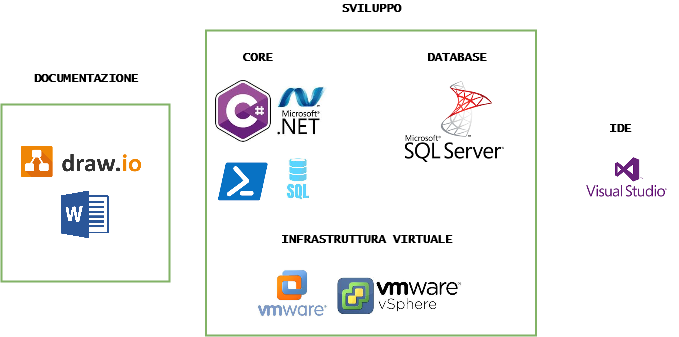
\includegraphics[width=0.7\textwidth ]{figures/tecno.png}
            \caption [Teconologie stage]{Schema di utilizzo delle tecnologie nel progetto di stage \label{fig:tecnologie}}
    \end{figure}
    

\section{Struttura del Documento}
Il resto della relazione di fine stage si divide nei seguenti capitoli:
\begin{itemize}
    \item Capitolo 2: contiene la descrizione del progetto aziendale e delle motivazioni che hanno portato l’azienda a desiderare lo stage svolto. Viene analizzato il contesto in cui si colloca, le aspettative dell’azienda e i vincoli da rispettare;
    \item Capitolo 3: contiene la descrizione dello stage e dei risultati e attività svolte per conseguirli;
    \item Capitolo 4: contiene la valutazione retrospettiva dello stage.
\end{itemize}

\section{Convenzioni tipografiche}
All’interno del documento vengono utilizzate le seguenti convenzioni tipografiche:
\begin{itemize}
    \item \emph{Corsivo}: indica i termini in lingua straniera o facenti parti del linguaggio tecnico;
    \item \gl{Termine} : indica i termini per cui viene fornita una definizione nel glossario. Viene sottolineata solamente la prima occorrenza del termine;
    \item {[1]}: indica i riferimenti bibliografici.
\end{itemize}